\documentclass[12pt]{scrartcl}
\usepackage{graphicx}
\graphicspath{{./}}
\usepackage[sexy]{evan}
\usepackage[normalem]{ulem}
\usepackage{hyperref}
\usepackage{mathtools}
\usepackage{multicol}
\hypersetup{
    colorlinks=true,
    linkcolor=blue,
    filecolor=magenta,      
    urlcolor=cyan,
    pdfpagemode=FullScreen,
    }
\usepackage[most]{tcolorbox}
\renewcommand{\dangle}{\measuredangle}

\renewcommand{\baselinestretch}{1.5}

\addtolength{\oddsidemargin}{-0.4in}
\addtolength{\evensidemargin}{-0.4in}
\addtolength{\textwidth}{0.8in}
% \addtolength{\topmargin}{-0.2in}
% \addtolength{\textheight}{1in} 


\setlength{\parindent}{0pt}

\usepackage{pgfplots}
\pgfplotsset{compat=1.15}
\usepackage{mathrsfs}
\usetikzlibrary{arrows}

\title{WMI Final 2024 - Simulation 2}
\author{Question Paper}
\date{17.00 WIB, 8 July 2024 - 17.00 WIB, 10 July 2024}

\begin{document}
\maketitle
\begin{center}
    \Huge
    \boxed{\textbf{Grade 5 - 6}}
\end{center}
\vspace{3cm}

\begin{flushleft}
\LARGE
   Total time allowed: 90 minutes\\
\large
   Section A : 40 minutes\\
   Break : 10 minutes\\
   Section B : 40 minutes
\end{flushleft}

\vspace{2cm}
\begin{flushleft}
    \Large
    \textbf{Link to submit the answers:} \url{https://forms.gle/uJ4hNjkm73DnAqmb8}
\end{flushleft}

\newpage
\section*{Simulation Rules}

\begin{enumerate}[leftmargin=*]
    \item There will be \textbf{NO Zoom meeting} for this simulation. Students are going to do it by themselves.
    
    \item Question papers are going to be uploaded to Google Drive at around 4-5 PM on the day of the simulation. Students may print or download the question paper.
    
    \item There are 25 questions in total.
    \begin{itemize}
        \item Section A consists of 15 Multiple Choice Questions. Problems 1-10 score 6 points each. Problems 11-15 score 8 points each. No points are deducted for unanswered question or wrong answer.
        \item Section B consists of 10 Open-Ended Questions. They score 10 points each, no points are deducted for unanswered or wrong answer.
    \end{itemize}

    \item \textbf{Total time: 90 minutes} 
    \newline
    Section A : 40 minutes.\\
    Break : 10 minutes \\
    Section B : 40 minutes.
    
    Students are advised to set a timer to ensure the timing is accurate and is according to the actual condition during WMI Finals 2024.
    
    \item In order to have the best simulation experience, students are advised to have necessary stationery, blank papers (to scribble), and bottled water.
    
    \item No calculators, smart watches/digital watches and digital dictionaries are allowed.
    
    \item Submission can be done by filling in Google Forms. The links of the Google Forms are on the 1st pages of each question paper.
    
    \item Students may only submit once. If there are multiple submissions, only the first one will be considered.
    
    \item Please submit the answers by Wednesday, 10 July 2024, 17:00 WIB. Late submissions will still be marked, but not included in the ranking.
    
    \item The scores are going to be announced during the class on Wednesday, 10 July 2024.
\end{enumerate}

\pagestyle{plain}
\newpage
\section{Section A}
\subsection*{Problems 1-10. Six points each. Choose the best answer from (A) -- (D).}
\hrulefill

\begin{enumerate}
\item $9 \times 0.1 + 17 \times 0.02 = ?$
    \begin{multicols}{4}
        \begin{enumerate}[(A)]
            \item 1.04
            \item 1.07
            \item 1.24
            \item 1.34
        \end{enumerate}
    \end{multicols} \hrulefill

\item Which number below has the most factors?
    \begin{multicols}{4}
        \begin{enumerate}[(A)]
            \item 169
            \item 98
            \item 90
            \item 62
        \end{enumerate}
    \end{multicols} \hrulefill

\item $60500\text{\textit{cc}} = (\ldots)\text{ \textit{l} }(\ldots)\text{\textit{ml}}$
    \begin{multicols}{4}
        \begin{enumerate}[(A)]
            \item 60 \textit{l} 500 \textit{ml}
            \item 6 \textit{l} 5000 \textit{ml}
            \item 6 \textit{l} 500 \textit{ml}
            \item 6 \textit{l} 50 \textit{ml}
        \end{enumerate}
    \end{multicols} \hrulefill

\item Unfold the solids below. Which has the most rectangles?
        \begin{multicols}{4}
        \begin{enumerate}[(A)]
            \item 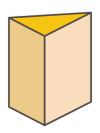
\includegraphics[scale=0.5]{StarGen/0Figure/wmi-2020-5a-4-a.png}
                    
            \item 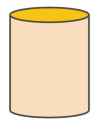
\includegraphics[scale=0.95]{StarGen/0Figure/wmi-2020-5a-4-b.png}
                    
            \item 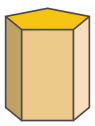
\includegraphics[scale=0.5]{StarGen/0Figure/wmi-2020-5a-4-c.png}
                    
            \item 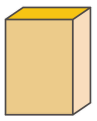
\includegraphics[scale=0.5]{StarGen/0Figure/wmi-2020-5a-4-d.png}  
        \end{enumerate}
        \end{multicols} \hrulefill
\hrulefill

\item $(125 \times 6) \div 5 + (75 \times 5) \div 3 = ?$
    \begin{multicols}{4}
        \begin{enumerate}[(A)]
            \item 200
            \item 245
            \item 275
            \item 295
        \end{enumerate}
    \end{multicols} \hrulefill

\newpage
\item $57.132 = ?$
        \begin{enumerate}[(A)]
            \item $5 \times 10 + 7 \times 1 + 2 \times \frac{1}{1000} + 3 \times \frac{1}{100} + 1 \times \frac{1}{10}$
            \item $5 \times 10 + 7 \times 1 + 1 \times \frac{1}{1000} + 3 \times \frac{1}{100} + 2 \times \frac{1}{10}$
            \item $5 \times 10 + 7 \times 1 + 3 \times \frac{1}{1000} + 2 \times \frac{1}{100} + 1 \times \frac{1}{10}$
            \item $5 \times 10 + 3 \times 1 + 2 \times \frac{1}{1000} + 3 \times \frac{1}{100} + 1 \times \frac{1}{10}$
        \end{enumerate} \hrulefill

\item Find the shaded area of the figure in cm$^2$.
    \begin{figure}[h]
        \centering
        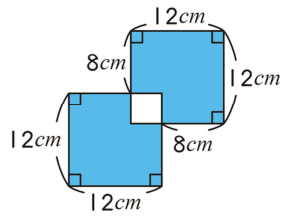
\includegraphics[scale=0.7]{StarGen/0Figure/wmi-2020-5a-7.png}
    \end{figure}
    \begin{multicols}{4}
        \begin{enumerate}[(A)]
            \item 288
            \item 280
            \item 272
            \item 256
        \end{enumerate}
    \end{multicols} \hrulefill

\item Harden is a famous shooter in the NBA, and his three-point field goal percentage is $x\%$ in this year. If he makes 843 three-pointers this year, how many of them score?
    \begin{multicols}{4}
        \begin{enumerate}[(A)]
            \item $843x$
            \item $8.43x$
            \item $3x$
            \item $0.3x$
        \end{enumerate}
    \end{multicols} \hrulefill

\item $\dfrac{4}{5} : \dfrac{3}{4} = 32 : \square$, $\square = ?$
    \begin{multicols}{4}
        \begin{enumerate}[(A)]
            \item 24
            \item 28
            \item 30
            \item 40
        \end{enumerate}
    \end{multicols} \hrulefill

\newpage
\item The volume of a cuboid is 108cm$^3$. If its length and width are 8cm and $2\frac{1}{4}$cm, respectively, find its height in cm.
    \begin{multicols}{4}
        \begin{enumerate}[(A)]
            \item 6
            \item 7
            \item 8
            \item 9
        \end{enumerate}
    \end{multicols} \hrulefill
\end{enumerate}

\subsection*{Problems 11-15. Eight points each. Choose the best answer from (A) -- (D).}
\hrulefill

\begin{enumerate}[resume]
\item Ann computes $36 + 14 \times (8 - 5)$. Is the process "correct" ($v$)? Or, does a "mistake" ($x$) occur at a certain step?
        \begin{figure}[h]
            \centering
            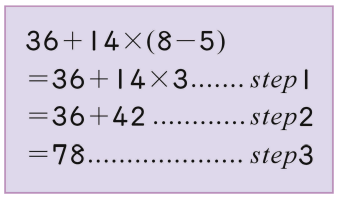
\includegraphics[scale=0.5]{StarGen/0Figure/wmi-2020-5a-11.png}
        \end{figure}
    \begin{multicols}{4}
        \begin{enumerate}[(A)]
            \item $v$
            \item $x$, step 1
            \item $x$, step 2
            \item $x$, step 3
        \end{enumerate}
    \end{multicols} \hrulefill

\item Find the surface area of the solid in cm$^2$.
    \begin{figure}[h]
        \centering
        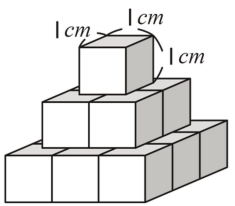
\includegraphics[scale=0.6]{StarGen/0Figure/wmi-2020-5a-12.png}
    \end{figure}
    \begin{multicols}{4}
        \begin{enumerate}[(A)]
            \item 36
            \item 42
            \item 45
            \item 54
        \end{enumerate}
    \end{multicols} \hrulefill

\newpage
\item Among fractions whose denominators are 18, how many of them are larger than $\frac{1}{6}$ yet smaller than $\frac{4}{9}$?
    \begin{multicols}{4}
        \begin{enumerate}[(A)]
            \item 8
            \item 6
            \item 5
            \item 4
        \end{enumerate}
    \end{multicols} \hrulefill

\item Given a large square on the right. Find $x$ in cm.
    \begin{figure}[h]
        \centering
        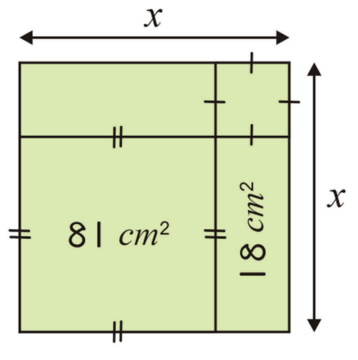
\includegraphics[scale=1]{StarGen/0Figure/wmi-2020-5a-square.png}
    \end{figure}
    \begin{multicols}{4}
        \begin{enumerate}[(A)]
            \item 13
            \item 12
            \item 11
            \item 10
        \end{enumerate}
    \end{multicols} \hrulefill

\item How many numbers satisfy the three conditions below?
\begin{itemize}
    \item[(i)] A 3-digit number which is larger than 700.
    \item[(ii)] A multiple of 11.
    \item[(iii)] Not a multiple of 2.
\end{itemize}
    \begin{multicols}{4}
        \begin{enumerate}[(A)]
            \item 24
            \item 15
            \item 13
            \item 12
        \end{enumerate}
    \end{multicols} \hrulefill
\end{enumerate}

\newpage
\section{Section B}
\subsection*{Ten points each. \textbf{No need to write down any units.} All answers are guaranteed in integer form.}
\hrulefill
\begin{enumerate}[resume]
\item $2-(2+4)+(2+4+6)-(2+4+6+8)+\cdots-(2+4+\cdots+96)+(2+4+\cdots+98)=?$

\hrulefill \item If both $n-1$ and $n+1$ are primes, the positive integer $n$ is called a "prime interlude". Find the number of "prime interludes" among 2-digit numbers.

\hrulefill \item Write figures 1, 2, 3, 4, 5, 6, 7, 8, and 9 into the squares in a different order to make the sum of each set of upper figure and lower figure a perfect square. How do these 9 figures arranged from left to right?
    \begin{figure}[h]
        \centering
        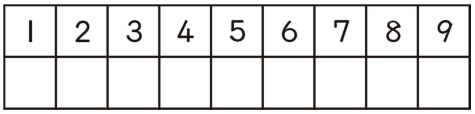
\includegraphics[scale=0.6]{StarGen/0Figure/wmi-2020-5b-3.png}
    \end{figure}

\hrulefill \item Suppose $A \bowtie B = A \times B + A + B$. Find $(20 \bowtie 20) \bowtie (20 \bowtie 20)$.

\hrulefill \item The figure is formed by a regular hexagon, 6 squares, and 6 small regular triangles. Given that the area of $\triangle ABC$ is 12cm$^2$, find the sum of the areas of the 6 shaded small regular triangles in cm$^2$.
    \begin{figure}[h]
        \centering
        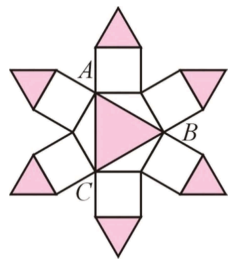
\includegraphics[scale=1]{StarGen/0Figure/wmi-2020-5b-5.png}
    \end{figure}

\hrulefill \item Delete 6 of the 16 figures in the squares so that the numbers of the figures on each row and each column are even numbers. Find the maximum sum of the remaining 10 numbers.
    \begin{figure}[h]
        \centering
        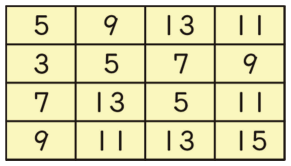
\includegraphics[scale=0.7]{StarGen/0Figure/wmi-2020-5b-6.png}
    \end{figure}

\hrulefill \item Fill up a container with water. Put iron ball A in the container and take it out. Then, put iron ball B in the container and take it out. In the end, put iron ball C in the container. Given that the amount of spilling water at the second time is $\frac{1}{3}$ of the amount of spilling water at the first time, and the amount of spilling water at the third time is twice the amount of spilling water at the first time. If the volume of iron ball A is 30cm$^3$, find the volume of iron ball C in cm$^3$.

\hrulefill \item Take 9 numbers from 1--20 without repetition and fill them in a $3 \times 3$ grid so that the sums on each row, each column, and each diagonal are the same. If there are $a$ primes among these 9 numbers at most, and that the largest prime is $b$, find $a \times b$.
    \begin{figure}[h]
        \centering
        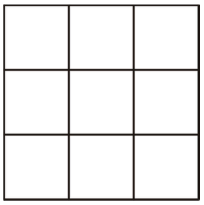
\includegraphics[scale=0.5]{StarGen/0Figure/wmi-2020-5b-8.png}
    \end{figure}

\hrulefill \item Given 4 different positive integers $a$, $b$, $c$, and $d$ that satisfy $\frac{1}{a} + \frac{1}{b} + \frac{1}{c} + \frac{1}{d} = 1$. Find the minimum value of $a+b+c+d$.

\hrulefill \item The picture shows a Sudoku game with number 1 to 5. The number and the math symbol in the top left corner of the frame indicate the result in each frame. For example, "6+" means that the sum of the numbers in the frame is 6. Find the 5-digit number $\overline{ABCDE}$.
    \begin{figure}[h]
        \centering
        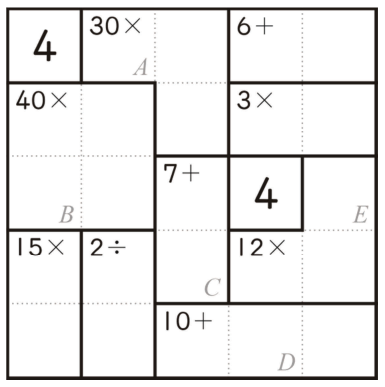
\includegraphics[scale=0.5]{StarGen/0Figure/wmi-2020-5b-10.png}
    \end{figure}
    
\hrulefill
\end{enumerate}


\end{document}